\documentclass[12pt,a4paper]{article}
\usepackage[utf8]{inputenc}
\usepackage[spanish]{babel}
\usepackage{amsmath}
\usepackage{amsfonts}
\usepackage{amssymb}
\usepackage{graphicx}
\usepackage[left=2cm,right=2cm,top=2cm,bottom=2cm]{geometry}

%--------------------------------------------------------%
%         Paquetes usados sólo para esta entrega         %
%--------------------------------------------------------%

\usepackage[hidelinks]{hyperref}
\usepackage{algorithm}
\usepackage{algorithmic}
\usepackage{float}




\author{Ignacio Aguilera Martos \\
	DNI: 77448262V       e-mail: nacheteam@correo.ugr.es \\
	Grupo de prácticas 1 Lunes 17:30-19:30}
\title{Práctica Algoritmos de Trayectorias \\ Metaheurísticas}
\date{Curso 2017-2018}

%Quita la sangría
\setlength{\parindent}{0cm}


\begin{document}
	\maketitle

	\tableofcontents

	\newpage

	%p 56

%	\framebox[16cm][c]{\LaTeX}

	\section{Introducción del problema}
	\label{sec:introProblema}

	Para el problema de clasificación partimos de un conjunto de datos dado por una serie de tuplas que contienen los valores de atributos para cada instancia. Esto es una n-tupla de valores reales en nuestro caso.
	
	El objetivo del problema es obtener un vector de pesos que asocia un valor en el intervalo $[0,1]$ indicativo de la relevancia de ese atributo. Esta relevancia va referida a lo importante que es en nuestro algoritmo clasificador ese atributo a la hora de computar la distancia entre elementos.
	
	Resumiendo lo que tenemos es un algoritmo clasificador que utiliza el vector de pesos calculado para predecir la clase a la que pertenece una instancia dada. Este algoritmo clasificador es el KNN con k=1. Lo que hace es calcular según la distancia euclídea (o cualquier otra) la tupla más cercana a la que queremos clasificar ponderando cada atributo con el correspondiente peso del vector, es decir, la distancia entre dos elementos sería:
	$$d(e,f) = \sqrt{\sum_{i=0}^{n}w_i * (e_{i} - f_{i})}$$
	Donde e y f son instancias del conjunto de datos, w el vector de pesos y n la longitud de e y f que es la misma.
	
	La calificación que se le asigna al vector w depende de dos cosas: la tasa de aciertos y la simplicidad.
	
	La tasa de aciertos se mide contando el número de aciertos al emplear el clasificador descrito y la simplicidad se mide como el número de elementos del vector de pesos que son menores que 0.2, ya que estos pesos no son empleados por el clasificador, o lo que es lo mismo, son sustituidos por cero. Por lo tanto las calificaciones siguen las fórmulas:
	$$Tasa\_acierto = 100\cdot \frac{nº  \ aciertos}{nº \ datos} \ , \ Tasa\_simplicidad = 100\cdot \frac{nº \ valores \ de \ w \ < \ 0.2}{nº \ de \ atributos}$$
	$$Tasa\_agregada = \frac{1}{2}\cdot Tasa\_acierto + \frac{1}{2}\cdot Tasa\_simplicidad$$
	Cabe destacar que todas las tasas están expresadas en porcentajes, por lo tanto cuanto más cercano sea el valor a 100 mejor es la calificación.
	
	De esta forma a través del algoritmo que obtiene el vector de pesos para el conjunto de datos dado y el clasificador obtenemos un programa que clasifica de forma automática las nuevas instancias de datos que se introduzcan.


	\section{Introducción de la práctica}
	\label{sec:introPractica}

	En esta práctica se analizan los algoritmos Enfriamiento Simulado, ILS y Evolución diferencial.
	
	Al igual que en las prácticas anteriores se van a poner en contraposición al resto de algoritmos para comparar cómo mejoran o empeoran los resultados y sacar conclusiones sobre los mismos.
	
	Cabe destacar que no hay repetición de tuplas en los conjuntos de datos utilizados, ya que he realizado un preprocesamiento en la lectura para eliminar tuplas con los mismos valores. 
	
	Así mismo cabe destacar que he reutilizado la búsqueda local implementada en la primera práctica para el desarrollo del algoritmo ILS.
	
	De igual modo he implementado Evolución Diferencial con dos operadores de mutación (Rand1 y Current to Best 1) tal y como se detallará en la correspondiente sección.

	\newpage

	\section{Descripción común a todos los algoritmos}

	Los algoritmos empleados han sido el KNN, el algoritmo greedy Relief, la metaheurística de búsqueda local, un algoritmo genético estacionario, un algoritmo genético generacional, un memético basado en el algoritmo genético generacional, enfriamiento simulado, ILS y evolución diferencial.
	
	Estos algoritmos comparten ciertos métodos y operadores que pasaré a explicar en esta sección.
	
	Para empezar se debe destacar que la representación escogida para las soluciones es un vector de números reales, es decir, si n es el número de características:
	$$w\in \mathbb{R}^n \ t.q. \ \forall i \ con \ 0\leq i < n \ se \ tiene \ w_i \in [0,1]$$
	O lo que es lo mismo, un vector de tamaño n con todas las posiciones rellenas con números del intervalo [0,1].
	
	A estos números me referiré como pesos asociados a las características, ya que lo que nos indican es el grado de importancia de dicha característica a la hora de clasificar los datos, siendo 1 el máximo de relevancia y 0 el mínimo.
	
	Así mismo cabe destacar que nuestra intención en este problema es obtener una buena calificación de dicho vector de pesos. Esto lo medimos mediante las tasas de acierto y simplicidad que se definen como:
	$$Tasa\_acierto = 100\cdot \frac{nº  \ aciertos}{nº \ datos} \ , \ Tasa\_simplicidad = 100\cdot \frac{nº \ valores \ de \ w \ < \ 0.2}{nº \ de \ atributos}$$
	$$Tasa\_agregada = \frac{1}{2}\cdot Tasa\_acierto + \frac{1}{2}\cdot Tasa\_simplicidad$$
	
	La tasa de aciertos lo que nos mide es en un porcentaje cuántas instancias hemos clasificado correctamente mediante el algoritmo KNN usando el vector de pesos w.
	
	La tasa de simplicidad nos mide cuántos de los valores que tiene el vector de pesos son menores que 0.2. Esto se hace ya que, como imposición del problema, tenemos que si alguno de los pesos es menor que 0.2 no debemos usarlo, o lo que es lo mismo, debemos sustituirlo por un 0 en la función de la distancia que luego describiré. Midiendo esto obtenemos un dato de cuanto sobreajuste ha tenido nuestro algoritmo a la hora de obtener el vector de pesos. Cuantas menos características necesitemos para discernir la clase a la que pertenece una instancia de los datos, más simple será clasificar dicha instancia. Se expresa en porcentaje indicando 0 como ninguna simplicidad y 100 como la máxima simplicidad.
	
	De esta forma combinando ambas tasas obtenemos la tasa agregada que nos hace la media entre ambas tasas, de forma que le asignamos la misma importancia a acertar en la clasificación de las instancias y a la simplicidad en la solución. Cabe destacar que es imposible obtener una tasa de un 100\% a no ser que los datos se compongan únicamente de un punto ya que ello implicaría que la simplicidad ha de ser un 100\% (todos las posiciones del vector menores que 0.2) y por tanto la distancia sería 0 en todos los casos. De esta forma aspiraremos a una calificación lo mas alta posible pero teniendo en cuenta las restricciones de la función objetivo construida.
	
	Las funciones y operadores de uso común los he agrupado en un fichero llamado auxiliar.py. Este fichero contiene las funciones de lectura de datos, distancias, una función que devuelve el elemento más común de una lista, la norma euclídea, una función para dividir los datos en el número de particiones que queramos manteniendo el porcentaje de elementos de cada clase que había en el conjunto de datos original y el operador de mutación básico.
	
	\subsection{Generación de soluciones aleatorias}
	
	En el algoritmo DE partimos de una población de soluciones aleatorias que generamos con una distribución uniforme, de forma que partimos en un inicio con una población de 50 individuos con valores en los vectores de pesos entre 0 y 1 generados de forma aleatoria.
	
	Nótese que en nuestro caso TAM\_POBLACION=50.
	
	\begin{algorithm}
		\caption{generaPoblacionInicial(longitud)}
		\begin{algorithmic}
			\STATE poblacion $\leftarrow$ [ ]
			\FOR{i=0 , ... , TAM\_POBLACION-1}
			\STATE cromosoma $\leftarrow$ [ ]
			\FOR{j=0 , ... , longitud-1}
			\STATE cromosoma $\leftarrow$ [cromosoma,uniforme(0,1)]
			\ENDFOR
			\STATE poblacion $\leftarrow$ [poblacion,cromosoma]
			\ENDFOR
			\RETURN poblacion
		\end{algorithmic}
	\end{algorithm}

	\newpage
	
	\section{Enfriamiento Simulado}
	\label{sec:ES}
	
	El algoritmo de enfriamiento simulado basa su comportamiento en varios factores numéricos entre los que podemos encontrar a la temperatura inicial, temperatura final y el esquema de enfriamiento que nos va a indicar cuanta exploración y explotación va a tener el algoritmo en función de la solución inicial conseguida.
	
	En primer lugar la temperatura inicial la calculamos con las constantes $\mu$ y $\phi$ que vienen determinadas mediante el guión por el valor 0.3 ambas. Esto nos indica que tenemos probabilidad 0.3 de aceptar una solución un 30\% peor que la que estamos considerando actualmente.
	
	A raíz de esto podemos definir la temperatura inicial como $T0 = \frac{\mu  \cdot C(S_0)}{-\log(\phi)}$ donde $C(S_0)$ es el coste de la solución inicial.
	
	Así mismo definimos la temperatura final como $TF=10^{-3}$. Como podemos tener la casuística de que desde el inicio del algoritmo la temperatura inicial ya sea menor que la final he definido la temperatura final como $TF=10^{-3}$ si esta constante es menor que la temperatura inicial o como $TF=T0-10^{-3}$ para tener así un margen de aplicación del algoritmo.
	
	El esquema de enfriamiento propuesto ha sido el esquema de enfriamiento de Cauchy modificado que nos otorga una convergencia mayor al decrementar la temperatura de forma más rápida que una lineal. Estas dos formas serán comparadas posteriormente en el análisis de resultados. El esquema de enfriamiento de Cauchy viene dado por las fórmulas:
	
	\vspace{10px}
	
	$\beta = \frac{T_0 - T_f}{M\cdot T_0\cdot T_f}$
	
	\vspace{10px}
	
	$T_{k+1} = \frac{T_k}{1+\beta \cdot T_k}$
	
	\vspace{10px}
	
	Donde M es el número de enfriamientos a realizar.
	
	A parte de estas constantes debemos tener en cuenta que el algoritmo está limitado a 15000 evaluaciones y el procedimiento de enfriamiento se aplica cuando hemos visitado $10\cdot D$ vecinos donde D es la dimensión del problema o cuando se han aceptado $0.1\cdot 10\cdot D$ vecinos como soluciones por el procedimiento.
	
	A continuación se describe el algoritmo en pseudocódigo: 
	
	\begin{algorithm}
		\caption{EnfriamientoSimulado(data,k,MAX\_EVALS)}
		\begin{algorithmic}
			\STATE ncar $\leftarrow$ número de características
			\STATE sol  $\leftarrow$ solución inicial aleatoria
			\STATE valoracion $\leftarrow$ valoración de la solución inicial
			\STATE mejor\_sol $\leftarrow$ sol
			\STATE valoracion\_mejor\_sol $\leftarrow$ valoracion
			\STATE
			\STATE $T_0$ $\leftarrow$ $\frac{\mu  \cdot C(S_0)}{-\log(\phi)}$
			\STATE
			\IF{T0$<$$10^{-3}$}
				\STATE $T_f$ $\leftarrow$ $10^{-3}$
			\ELSE
				\STATE $T_f$  $\leftarrow$ T0-$10^{-3}$
			\ENDIF
			\STATE max\_vecinos $\leftarrow$ 10*ncar
			\STATE M $\leftarrow$ $\frac{MAX\_EVALS}{max\_vecinos}$
			\STATE max\_exitos $\leftarrow$ 0.1*max\_vecinos
			\STATE
			\STATE $\beta$ $\leftarrow$ $\frac{T_0-T_f}{M*T_0*T_f}$
			\STATE
			\STATE t $\leftarrow$ $T_0$
			\STATE evaluaciones $\leftarrow$ 1
			\STATE K $\leftarrow$ 1
			\WHILE{t$>$$T_f$ and evaluaciones$<$MAX\_EVALS}
				\STATE vecinos $\leftarrow$ 0
				\STATE aceptados $\leftarrow$ 0
				\WHILE{aceptados$<$max\_exitos and vecinos$<$max\_vecinos}
					\STATE vecinos $\leftarrow$ vecinos + 1
					\STATE evaluaciones $\leftarrow$ evaluaciones + 1
					\STATE vecino $\leftarrow$ Mutación de una posición aleatoria
					\STATE valoracion\_vecino $\leftarrow$ Valoración del vecino
					\STATE delta $\leftarrow$ valoracion - valoracion\_vecino
					\IF{delta$<$0 or valorAleatorio(0,1)$<$exp(-delta/(t*K))}
						\STATE sol $\leftarrow$ vecino
						\STATE valoracion $\leftarrow$ valoracion\_vecino
						\STATE aceptados $\leftarrow$ aceptados + 1
						
						\IF{valoracion\_mejor\_sol$<$valoracion}
							\STATE mejor\_sol $\leftarrow$ sol
							\STATE valoracion\_mejor\_sol $\leftarrow$ valoracion
						\ENDIF
					\ENDIF
				\ENDWHILE
				\STATE t $\leftarrow$ t/(1.0+$\beta$*t)
				\STATE K $\leftarrow$ K+1
			\ENDWHILE
		\end{algorithmic}
	\end{algorithm}
	
	\newpage
	
	\section{Búsqueda Local Reiterada}
	\label{sec:ILS}
	
	La búsqueda local reiterada es un algoritmo que se basa en realizar mutaciones a una solución e ir aplicando el algoritmo de búsqueda local a estas soluciones mutadas quedándote con la mejor de ellas en el proceso.
	
	La intención de este algoritmo es realizar un reinicio controlado de las soluciones e ir aplicando la búsqueda local a estas soluciones pseudoaleatorias (no son aleatorias puras ya que son una mutación de una solución aleatoria mejorada con búsqueda local).
	
	Estas mutaciones permiten al algoritmo simple de búsqueda local escaparse de los máximos locales ya que en el proceso de mutación podemos obtener una solución peor que la actual y luego mejorarla mediante el uso de la búsqueda local.
	
	El procedimiento de mutación es similar al usado en los algoritmos genéticos y el usado durante todo el desarrollo de las tres prácticas.
	
	A continuación se describe en pseudocódigo las funciones empleadas en la mutación:
	
	\begin{algorithm}
		\caption{mutacionILS(solucion,MU=0,SIGMA=0.4)}
		\begin{algorithmic}
			\STATE num\_mutaciones $\leftarrow$ 0.1*longitud(solucion)
			\STATE sample $\leftarrow$ num\_mutaciones índices aleatorios sin repetición entre 0 y logitud(solucion)
			\FOR{i en sample}
				\STATE solucion $\leftarrow$ mutacion(solucion,i,MU,SIGMA)
			\ENDFOR		
			\RETURN solucion
		\end{algorithmic}
	\end{algorithm}
	
	\begin{algorithm}
		\caption{mutacion(w,pos,MU,SIGMA)}
		\begin{algorithmic}
			\STATE incremento $\leftarrow$ gauss(MU,SIGMA)
			\STATE w[pos] $\leftarrow$ w[pos] + incremento
			\IF{w[pos]$<$0}
				\STATE w[pos] $\leftarrow$ 0
			\ELSIF{w[pos]$>$1}
				\STATE w[pos] $\leftarrow$ 1
			\ENDIF
			\RETURN w
		\end{algorithmic}
	\end{algorithm}
	
	A continuación describo el pseudocódigo de ILS:
	
	\begin{algorithm}
		\caption{ILS(data,k,MAX\_EVALS)}
		\begin{algorithmic}			
			\STATE ncar $\leftarrow$ longitud(data[0])
			\STATE mejor\_solucion $\leftarrow$ [0,0,...,0]
			\STATE valoracion\_mejor\_solucion $\leftarrow$ 0
			\STATE evaluaciones $\leftarrow$ 1
			\WHILE{evaluaciones $<$ MAX\_EVALS}
				\STATE solucion $\leftarrow$ Solución aleatoria
				\STATE valoracion $\leftarrow$ Valoracion(solucion)
				\IF{valoracion$>$valoracion\_mejor\_solucion}
					\STATE mejor\_solucion $\leftarrow$ solucion
					\STATE valoracion\_mejor\_solucion $\leftarrow$ valoracion
				\ENDIF
				\STATE mejorada,ev $\leftarrow$ busquedaLocal(data,k,1000,solucion)
				\STATE evaluaciones $\leftarrow$ evaluciones + ev
				\STATE valoracion\_mejorada $\leftarrow$ Valoracion(mejorada)
				\IF{valoracion\_mejorada$>$valoracion\_mejor\_solucion}
					\STATE mejor\_solucion $\leftarrow$ mejorada
					\STATE valoracion\_mejor\_solucion $\leftarrow$ valoracion\_mejorada
				\ENDIF
				\IF{valoracion $>$ valoracion\_mejorada}
					\STATE mejor\_local $\leftarrow$ solucion
					\STATE valoracion\_mejor\_local $\leftarrow$ valoracion
				\ELSE
					\STATE mejor\_local $\leftarrow$ mejorada
					\STATE valoracion\_mejor\_local $\leftarrow$ valoracion\_mejorada
				\ENDIF
				\STATE evaluaciones $\leftarrow$ evaluaciones + 1
				\IF{valoracion\_mejor\_local$>$valoracion\_mejor\_solucion}
					\STATE mejor\_solucion $\leftarrow$ mejor\_local
					\STATE valoracion\_mejor\_solucion $\leftarrow$ valoracion\_mejor\_local
				\ENDIF
				\FOR{i en [0,...,13]}
					\STATE mutada $\leftarrow$ mutacionILS(mejor\_local)
					\STATE valoracion\_mutada $\leftarrow$ Valoracion(mutada)
					\STATE mutada\_mejorada,ev $\leftarrow$ busquedaLocal(data,k,1000,mutada)
					\STATE valoracion\_mutada\_mejorada $\leftarrow$ Valoracion(mutada\_mejorada)
					\STATE evaluaciones $\leftarrow$ evaluaciones + 2 + ev
					\IF{valoracion\_mutada$>$valoracion\_mutada\_mejorada}
						\STATE mejor\_local $\leftarrow$ mutada
						\STATE valoracion\_mejor\_local $\leftarrow$ valoracion\_mutada
					\ELSE
						\STATE mejor\_local $\leftarrow$ mutada\_mejorada
						\STATE valoracion\_mejor\_local $\leftarrow$ valoracion\_mutada\_mejorada
					\ENDIF
					
					\IF{valoracion\_mejor\_local$>$valoracion\_mejor\_solucion}
						\STATE mejor\_solucion $\leftarrow$ mejor\_local
						\STATE valoracion\_mejor\_solucion $\leftarrow$ valoracion\_mejor\_local
					\ENDIF
				\ENDFOR
			\ENDWHILE
			\RETURN mejor\_solucion
			
		\end{algorithmic}
	\end{algorithm}
	
	\newpage
	
	\section{Evolución Diferencial}
	\label{sec:DE}
	
	Este algoritmo es un algoritmo basado en la teoría de algoritmos genéticos haciendo un énfasis especial en la mutación y usando una recombinación diferente a posteriori. 
	
	Como podremos observar posteriormente en los resultados este es un algoritmo que arroja unos resultados muy buenos en el problema de selección de características.
	
	He implementado para este algoritmo dos modelos de mutación: Rand1 y Current to Best 1.
	
	Rand1 toma tres individuos aleatorios de la población para cada individuo al que queremos aplicar la mutación y devolvemos la suma del primer individuo aleatorio mas un factor de escala por la resta de los dos otros individuos generados.

	A continuación se describe el operador en pseudocódigo:
	
	\begin{algorithm}
		\caption{Rand1(individuo,poblacion,valoraciones)}
		\begin{algorithmic}			
			\STATE sample $\leftarrow$ [0,...,longitud(poblacion)] excluyendo al entero individuo
			\STATE Mezclamos de forma aleatoria la lista sample
			\STATE sample $\leftarrow$ 3 primeros elementos de sample
			\STATE
			\RETURN poblacion[sample[0]] + F*(poblacion[sample[1]]-poblacion[sample[2]])
		\end{algorithmic}
	\end{algorithm}
	
	Donde en nuestro caso $F=0.5$ como se sugiere en las diapositivas de teoría.
	
	El otro operador de mutación  es Current to Best 1 que se basa en intentar dirigir la mutación del individuo hacia el mejor actual de la población con un cierto factor de aleatoriedad al crear el individuo mutado usando dos individuos aleatorios de la población.
	
	A continuación se describe el pseudocódigo del operador:
	
	\begin{algorithm}
		\caption{CBT1(individuo,poblacion,valoraciones)}
		\begin{algorithmic}			
			\STATE sample $\leftarrow$ [0,...,longitud(poblacion)] excluyendo al entero individuo
			\STATE Mezclamos de forma aleatoria la lista sample
			\STATE sample $\leftarrow$ 2 primeros elementos de sample
			\STATE
			\STATE mejor $\leftarrow$ Índice del mejor elemento de la población
			\STATE
			\RETURN poblacion[individuo] + F*(poblacion[mejor] - poblacion[individuo]) + F*(poblacion[sample[0]] - poblacion[sample[1]])
		\end{algorithmic}
	\end{algorithm}
	
	Donde en nuestro caso $F=0.5$ como se sugiere en las diapositivas de teoría.
	
	En el algoritmo la mutación sólo la aplicamos si al generar un valor aleatorio este es menor que la constante CR que viene dada como la constante $CR = \frac{0.1}{0.9}$ en las diapositivas de teoría.
	
	Tras la mutación se hace la selección de los mejores para quedarnos con los de la generación anterior si no hemos mejorado o con los mutados si hemos obtenido mejora.
	
	A continuación se describe el algoritmo en pseudocódigo:
	
	\begin{algorithm}
		\caption{DE(data,k,operador\_mutacion,MAX\_EVALS=15000,TAM\_POBLACION=50)}
		\begin{algorithmic}			
			\STATE poblacion $\leftarrow$ Genera una población inicial aleatoria.
			\STATE valoraciones $\leftarrow$ Valoraciones de la población
			\STATE 
			\STATE evaluaciones $\leftarrow$ TAM\_POBLACION
			\STATE 
			\WHILE{evaluaciones$<$MAX\_EVALS}
				\STATE offspring $\leftarrow$ []
				\FOR{i en [0,...,TAM\_POBLACION-1]}
					\STATE random $\leftarrow$ Número aleatorio entre 0 y 1.
					\IF{random$<$CR}
						\STATE offspring $\leftarrow$ [offspring, operador\_mutacion(i,poblacion,valoraciones)]
					\ELSE
						\STATE offspring $\leftarrow$ [offspring,poblacion[i]]
					\ENDIF
				\ENDFOR
				\STATE valoraciones\_offspring $\leftarrow$ Valoraciones de la población offspring
				\STATE evaluaciones $\leftarrow$ evaluaciones + TAM\_POBLACION
				\STATE 
				\FOR{i en [0,...,TAM\_POBLACION-1]}
					\IF{valoraciones[i]$<$valoraciones\_offspring[i]}
						\STATE poblacion[i] $\leftarrow$ offspring[i]
						\STATE valoraciones[i] $\leftarrow$ valoraciones\_offspring[i]
					\ENDIF
				\ENDFOR
			\ENDWHILE
			\RETURN El mejor individuo de la población.
		\end{algorithmic}
	\end{algorithm}
	
	\newpage

	\section{Pseudocódigo Genético Estacionario}
	\label{sec:GE}


	\begin{algorithm}
		\caption{GeneticoEstacionario(data,k,operador\_cruce)}
		\begin{algorithmic}
			\STATE num\_padres $\leftarrow$ 0
			\IF{operador\_cruce == cruceAritmetico}
				\STATE num\_padres $\leftarrow$ 4
			\ELSIF{operador\_cruce == cruceBLX}
				\STATE num\_padres $\leftarrow$ 2
			\ELSE
				\STATE Error en el operador de cruce.
			\ENDIF
			\STATE
			\STATE poblacion $\leftarrow$ generaPoblacionInicial(numero\_caracteristicas)
			\STATE valoraciones $\leftarrow$ tasa\_agregada + tasa\_reduccion de cada individuo de la poblacion
			\STATE evaluaciones $\leftarrow$ TAM\_POBLACION
			\WHILE{evaluaciones $<$ MAX\_EVALUACIONES}
				\STATE padres $\leftarrow$ Padres escogidos por torneo binario según num\_padres
				\STATE hijos $\leftarrow$ Obtenemos los hijos según operador\_cruce con los padres calculados.
				\STATE
				\STATE Muta cada gen de los hijos si uniforme(0,1) es menor que 0.001.
				\STATE poblacion $\leftarrow$ [poblacion,hijos]
				\STATE valoraciones $\leftarrow$ [valoraciones,valoraciones de los hijos]
				\STATE Obtener los índices que los 30 mejores individuos de la población y quedarse con ellos.
				\STATE Actualizar poblacion y valoraciones según los índices obtenidos.
				\STATE evaluaciones $\leftarrow$ evaluaciones+2
			\ENDWHILE
			\RETURN Devolver al individuo con mayor valoración de la población.
		\end{algorithmic}
	\end{algorithm}

	\newpage

	\section{Peseudocódigo Genético Generacional}
	\label{sec:GG}

	\begin{algorithm}
		\caption{GeneticoGeneracional(data,k,operador\_cruce)}
		\begin{algorithmic}
			\STATE poblacion $\leftarrow$ generaPoblacionInicial(num\_caracteristicas)
			\STATE mutaciones $\leftarrow$ PROB\_MUTACION*TAM\_POBLACION*num\_caracteristicas
			\STATE num\_parejas $\leftarrow$ TAM\_POBLACION*PROB\_CRUCE
			\STATE valoraciones $\leftarrow$ valoraciones de la población
			\STATE mejor\_solucion $\leftarrow$ Mejor solución de la población.
			\WHILE{evaluaciones $<$ MAX\_EVALUACIONES}
				\STATE hijos $\leftarrow$ [ ]
				\FOR{i=0 , ... , num\_parejas-1}
					\IF{operador\_cruce==cruceAritmetico}
						\STATE padres $\leftarrow$ genera 4 padres con torneoBinario
						\STATE hijos $\leftarrow$ [hijos,operador\_cruce(padres[0],padres[1])]
						\STATE hijos $\leftarrow$ [hijos,operador\_cruce(padres[2],padres[3])]
						\STATE hijos $\leftarrow$ [hijos,operador\_cruce(padres[0],padres[2])]
						\STATE hijos $\leftarrow$ [hijos,operador\_cruce(padres[1],padres[2])]
					\ELSE
						\STATE padres $\leftarrow$ genera 2 padres con torneoBinario
						\STATE hijos $\leftarrow$ [hijos,operador\_cruce(padres[0],padres[1])]
						\STATE hijos $\leftarrow$ [hijos,operador\_cruce(padres[0],padres[1])]
					\ENDIF
				\ENDFOR
				\STATE Muta la nueva población de hijos con probabilidad 0.001 con una distribución $gauss(\mu=0,\sigma=0.3)$
				\STATE Rellena la población de hijos con padres haciendo torneos binarios.
				\STATE poblacion $\leftarrow$ hijos
				\STATE Actualiza las valoraciones de los individuos.
				\STATE Si el peor de la nueva población es peor que el mejor de la anterior lo sustituimos.
				\STATE Actualiza el mejor de la población.
			\ENDWHILE
			\RETURN Mejor de la población.
		\end{algorithmic}
	\end{algorithm}

	\newpage

	\section{Pseudocódigo Meméticos}
	\label{sec:memeticos}

	\begin{algorithm}
		\caption{Memetico(data,k,operador\_cruce,nGeneraciones,prob\_bl,mejores=False)}
		\begin{algorithmic}
			\STATE poblacion $\leftarrow$ generaPoblacionInicial(num\_caracteristicas)
			\STATE mutaciones $\leftarrow$ PROB\_MUTACION*TAM\_POBLACION*num\_caracteristicas
			\STATE num\_parejas $\leftarrow$ TAM\_POBLACION*PROB\_CRUCE
			\STATE valoraciones $\leftarrow$ valoraciones de la población
			\STATE mejor\_solucion $\leftarrow$ Mejor solución de la población.
			\STATE contador\_generaciones $\leftarrow$ 1
			\WHILE{evaluaciones $<$ MAX\_EVALUACIONES}
				\IF{contador\_generaciones\%nGeneraciones==0}
					\STATE n\_elem\_bl $\leftarrow$ prob\_bl*TAM\_POBLACION
					\STATE individuos $\leftarrow$ [ ]
					\IF{not mejores}
						\STATE individuos $\leftarrow$ Tomar n\_elem\_bl de forma aleatoria desde 0,...,TAM\_POBLACION-1
					\ELSE
						\STATE individuos $\leftarrow$ Toma los 0.1*TAM\_POBLACION mejores de la poblacion
					\ENDIF
					\FOR{ind en individuos}
						\STATE Aplica la búsqueda local a poblacion[ind]
						\STATE Actualiza el número de evaluaciones.
					\ENDFOR
					\STATE Actualiza las valoraciones
					\STATE Actualiza las evaluaciones.
				\ENDIF
				\STATE
				\STATE hijos $\leftarrow$ [ ]
				\FOR{i=0 , ... , num\_parejas-1}
					\IF{operador\_cruce==cruceAritmetico}
						\STATE padres $\leftarrow$ genera 4 padres con torneoBinario
						\STATE hijos $\leftarrow$ [hijos,operador\_cruce(padres[0],padres[1])]
						\STATE hijos $\leftarrow$ [hijos,operador\_cruce(padres[2],padres[3])]
						\STATE hijos $\leftarrow$ [hijos,operador\_cruce(padres[0],padres[2])]
						\STATE hijos $\leftarrow$ [hijos,operador\_cruce(padres[1],padres[2])]
					\ELSE
						\STATE padres $\leftarrow$ genera 2 padres con torneoBinario
						\STATE hijos $\leftarrow$ [hijos,operador\_cruce(padres[0],padres[1])]
						\STATE hijos $\leftarrow$ [hijos,operador\_cruce(padres[0],padres[1])]
					\ENDIF
				\ENDFOR
				\STATE Muta la nueva población de hijos con probabilidad 0.001 con una distribución $gauss(\mu=0,\sigma=0.3)$
				\STATE Rellena la población de hijos con padres haciendo torneos binarios.
				\STATE poblacion $\leftarrow$ hijos
				\STATE Actualiza las valoraciones de los individuos.
				\STATE Si el peor de la nueva población es peor que el mejor de la anterior lo sustituimos.
				\STATE Actualiza el mejor de la población.
				\STATE contador\_generaciones $\leftarrow$ contador\_generaciones + 1
			\ENDWHILE
			\RETURN Mejor de la población.
		\end{algorithmic}
	\end{algorithm}

	Donde prob\_bl es el porcentaje de la población al que queremos aplicar la búsqueda local.

	\newpage

	\section{Pseudocódigo KNN}
	\label{sec:knn}

	\begin{algorithm}
		\caption{KNN(w,datos\_test,datos\_entrenamiento, etiquetas\_entrenamiento, etiquetas\_test, k, mismos\_conjuntos)}
		\begin{algorithmic}
			\STATE tam\_datos\_entrenamiento $\leftarrow$ longitud(datos\_entrenamiento)
			\STATE clases $\leftarrow$ []
			\FOR{i=0,...,longitud(datos\_test)}
			\STATE p $\leftarrow$ datos\_test[i]
			\STATE w\_m $\leftarrow$ Repetir el vector w tantas veces como datos haya en datos\_entrenamiento.
			\STATE p\_m $\leftarrow$ Repetir el vector p tantas veces como datos haya en datos\_entrenamiento.
			\STATE dist $\leftarrow$ $w\_m \cdot (p\_m - datos\_entrenamiento)^2$
			\IF{mismos\_conjuntos}
			\STATE dist[i] $\leftarrow$ $\infty$
			\ENDIF
			\STATE mins $\leftarrow$ Los k índices correspondientes a las distancias más pequeñas.
			\STATE clases $\leftarrow$ [clases, masComun(etiquetas\_entrenamiento[mins])]
			\ENDFOR
			\RETURN $\frac{Numero \ de \ elementos \ de \ clases \ que \ han \ acertado \ con \ respecto \ a \ etiquetas\_test}{longitud(etiquetas\_test)}$
		\end{algorithmic}
	\end{algorithm}

	Cabe notar que el número que devolvemos está entre 0 y 1, por lo que en los algoritmos de valoración debemos tener esto en cuenta para multiplicarlo por 100 y convertirlo en un porcentaje.

	\newpage

	\section{Pseudocódigo Relief}
	\label{sec:relief}

	\begin{algorithm}
		\caption{elementoMinimaDistancia(e,lista)}
		\begin{algorithmic}
			\STATE distancias $\leftarrow$ [ ]
			\FOR{l en lista}
			\IF{l!=e}
			\STATE distancias $\leftarrow$ [distancias, distancia(e,l,[1..1])]
			\ELSE
			\STATE distancias $\leftarrow$ [distancias, max(distancias)]
			\ENDIF
			\ENDFOR
			\STATE indice\_menor\_distancia $\leftarrow$ índice del elemento de menor valor del vector distancias.
			\RETURN lista[indice\_menor\_distancia]
		\end{algorithmic}
	\end{algorithm}

	\begin{algorithm}
		\caption{Relief(data)}
		\begin{algorithmic}
			\STATE w $\leftarrow$ vector de pesos a 0
			\FOR{elemento en data}
			\STATE clase $\leftarrow$ clase de elemento
			\STATE amigos $\leftarrow$ [ ]
			\STATE enemigos $\leftarrow$ [ ]
			\FOR{e en data}
			\IF{e!=elemento AND e[longitud(e)-1]==clase}
			\STATE amigos $\leftarrow$ [amigos, e]
			\ELSE
			\STATE enemigos $\leftarrow$ [enemigos, e]
			\ENDIF
			\ENDFOR
			\STATE amigo\_cercano $\leftarrow$ elementoMinimaDistancia(elemento, amigos)
			\STATE enemigo\_cercano $\leftarrow$ elementoMinimaDistancia(elemento, enemigos)
			\STATE resta\_enemigo $\leftarrow$ element-enemigo\_cercano
			\STATE resta\_amigo $\leftarrow$ element-amigo\_cercano
			\STATE w $\leftarrow$ w + resta\_enemigo - resta\_amigo
			\STATE $w_{max}$ $\leftarrow$ máximo de w
			\ENDFOR
			\FOR{i en [0..longitud(w)-1]}
			\IF{w[i]$<$0}
			\STATE w[i] $\leftarrow$ 0
			\ELSE
			\STATE w[i] $\leftarrow$ $\frac{w[i]}{w_{max}}$
			\ENDIF
			\ENDFOR
			\RETURN w
		\end{algorithmic}
	\end{algorithm}

	\newpage

	\section{Pseudocódigo Búsqueda Local}
	\label{sec:bl}

	\begin{algorithm}
		\caption{primerVector(n)}
		\begin{algorithmic}
			\STATE w $\leftarrow$ [ ]
			\FOR{i en [0..n-1]}
			\STATE w $\leftarrow$ [w, random.uniforme(0,1)]
			\ENDFOR
			\RETURN w
		\end{algorithmic}
	\end{algorithm}

	\begin{algorithm}
		\caption{busquedaLocal(data,k)}
		\begin{algorithmic}
			\STATE MAX\_EVALUACIONES $\leftarrow$ 15000
			\STATE MAX\_VECINOS $\leftarrow$ $20\cdot longitud(data[0])$
			\STATE vecinos $\leftarrow$ 0
			\STATE evaluaciones $\leftarrow$ 0
			\STATE posicion\_mutacion $\leftarrow$ 0
			\STATE w $\leftarrow$ primerVector(longitud(data[0]))
			\STATE valoracion\_actual $\leftarrow$ Valoracion(data,data,k,w)
			\WHILE{evaluaciones$<$MAX\_EVALUACIONES AND vecinos$<$MAX\_VECINOS}
				\STATE evaluaciones $\leftarrow$ evaluaciones+1
				\STATE vecinos $\leftarrow$ vecinos+1
				\STATE vecino, posicion\_mutacion $\leftarrow$ mutacion(w,posicion\_mutacion)
				\STATE valoracion\_vecino $\leftarrow$ Valoracion(data,data,k,vecino)
				\IF{valoracion\_vecino$>$valoracion\_actual}
					\STATE vecinos $\leftarrow$ 0
					\STATE w $\leftarrow$ vecino
					\STATE valoracion\_actual $\leftarrow$ valoracion\_vecino
					\STATE posicion\_mutacion $\leftarrow$ 0
				\ELSIF{posicion\_mutacion==longitud(w)}
					\STATE posicion\_mutacion $\leftarrow$ 0
				\ENDIF
			\ENDWHILE
			\RETURN w
		\end{algorithmic}
	\end{algorithm}

	\newpage

	\section{Procedimiento de desarrollo de la práctica}
	\label{sec:procedimiento}

	La práctica ha sido desarrollada en Python3.5 utilizando la librería NumPy para agilizar los cálculos y que la computación fuera mucho más rápida.
	
	Los algoritmos están distribuidos en ficheros con extensión py con el mismo nombre que los algoritmos, de esta forma ILS estaría en el fichero ils.py por ejemplo.
	
	Si se quiere cambiar la semilla aleatoria esta se encuentra en la cabecera de los ficheros que albergan los algoritmos. 
	
	Si queremos obtener los resultados de todos los algoritmos implementados hasta ahora podemos ejecutar el fichero resultados.py de la siguiente forma:
	
	python3.5 resultados.py
	
	La ejecución de este fichero puede resultar excesivamente larga para comprobar un sólo algoritmo por lo que para ello he programado un fichero main.py que permite escoger el algoritmo que queremos ejecutar, el fichero de datos, la constante k de KNN y el número de particiones de los datos así como el algoritmo.
	
	Durante el transcurso de la práctica intenté utilizar el framework Sklearn pero lo encontré menos eficiente que las implementaciones que he realizado con NumPy por lo que descarté finalmente su uso.
	
	Por último cabe destacar que todo lo que es común a todos los algoritmos viene implementado en el fichero auxiliar.py donde podemos encontrar el algoritmo básico de mutación o la función de lectura de datos por ejemplo.

	\newpage

	\section{Resultados}
	\label{sec:resultados}

	\begin{table}[ht]
		\centering
		\resizebox{\textwidth}{!}{
			\begin{tabular}{| c | c | c | c | c | c | c | c | c | c | c | c | c |}
				\cline{2-13}
				\multicolumn{1}{c|}{} & \multicolumn{4}{|c|}{Ozone} & \multicolumn{4}{| c|}{Parkinsons} & \multicolumn{4}{|c|}{Spectf-Heart} \\ [0.5ex]
				\cline{2-13}
				\multicolumn{1}{c|}{} & \%\_clas & \%\_red & Agr. & T (seg) & \%\_clas & \%\_red & Agr. & T  (seg) & \%\_clas & \%\_red & Agr. & T  (seg) \\ [0.5ex] \hline
				Partición 1 & 71.8750 & 0.0000 & 35.9375 & 0.0111 & 76.3158 & 0.0000 & 38.1579 & 0.0032 & 70.5882 & 0.0000 & 35.2941 & 0.0072 \\ [0.5ex] \hline
				Partición 2 & 84.3750 & 0.0000 & 42.1875 & 0.0097 & 81.5789 & 0.0000 & 40.7895 & 0.0046 & 77.9412 & 0.0000 & 38.9706 & 0.0092 \\ [0.5ex] \hline
				Partición 3 & 71.8750 & 0.0000 & 35.9375 & 0.0095 & 94.7368 & 0.0000 & 47.3684 & 0.0031 & 67.6471 & 0.0000 & 33.8235 & 0.0083 \\ [0.5ex] \hline
				Partición 4 & 81.2500 & 0.0000 & 40.6250 & 0.0088 & 73.6842 & 0.0000 & 36.8421 & 0.0029 & 60.2941 & 0.0000 & 30.1471 & 0.0072 \\ [0.5ex] \hline
				Partición 5 & 85.9375 & 0.0000 & 42.9688 & 0.0089 & 76.7442 & 0.0000 & 38.3721 & 0.0032 & 66.2338 & 0.0000 & 33.1169 & 0.0071 \\ [0.5ex] \hline
				Media & 79.0625 & 0.0000 & 39.5313 & 0.0096 & 80.6120 & 0.0000 & 40.3060 & 0.0034 & 68.5409 & 0.0000 & 34.2704 & 0.0078 \\ [0.5ex] \hline
			\end{tabular}
		}
		\label{tabla1NN}
		\caption{Resultados 1NN}

	\end{table}



	\begin{table}[h!]
		\centering
		\resizebox{\textwidth}{!}{
			\begin{tabular}{| c | c | c | c | c | c | c | c | c | c | c | c | c |}
				\cline{2-13}
				\multicolumn{1}{c|}{} & \multicolumn{4}{|c|}{Ozone} & \multicolumn{4}{| c|}{Parkinsons} & \multicolumn{4}{|c|}{Spectf-Heart} \\ [0.5ex]
				\cline{2-13}
				\multicolumn{1}{c|}{} & \%\_clas & \%\_red & Agr. & T (seg) & \%\_clas & \%\_red & Agr. & T  (seg) & \%\_clas & \%\_red & Agr. & T  (seg) \\ [0.5ex] \hline
				Partición 1 & 64.0625 & 0.0000 & 32.0313 & 2.3071 & 76.3158 & 0.0000 & 38.1579 & 0.2821 & 26.4706 & 0.0000 & 13.2353 & 1.0612 \\ [0.5ex] \hline
				Partición 2 & 85.9375 & 0.0000 & 42.9688 & 1.6189 & 60.5263 & 0.0000 & 30.2632 & 0.2874 & 73.5294 & 0.0000 & 36.7647 & 1.0387 \\ [0.5ex] \hline
				Partición 3 & 75.0000 & 0.0000 & 37.5000 & 1.7513 & 76.3158 & 0.0000 & 38.1579 & 0.2792 & 73.5294 & 0.0000 & 36.7647 & 1.1519 \\ [0.5ex] \hline
				Partición 4 & 73.4375 & 0.0000 & 36.7188 & 1.7399 & 78.9474 & 0.0000 & 39.4737 & 0.2807 & 73.5294 & 0.0000 & 36.7647 & 1.0449 \\ [0.5ex] \hline
				Partición 5 & 81.2500 & 0.0000 & 40.6250 & 1.6257 & 72.0930 & 0.0000 & 36.0465 & 0.2769 & 29.8701 & 0.0000 & 14.9351 & 0.6444 \\ [0.5ex] \hline
				Media & 75.9375 & 0.0000 & 37.9688 & 1.8086 & 72.8397 & 0.0000 & 36.4198 & 0.2812 & 55.3858 & 0.0000 & 27.6929 & 0.9882 \\ [0.5ex] \hline
			\end{tabular}
		}
		\label{tablaReliefK1}
		\caption{Resultados Relief con K=1}
	\end{table}



	\begin{table}[h!]
		\centering
		\resizebox{\textwidth}{!}{
			\begin{tabular}{| c | c | c | c | c | c | c | c | c | c | c | c | c |}
				\cline{2-13}
				\multicolumn{1}{c|}{} & \multicolumn{4}{|c|}{Ozone} & \multicolumn{4}{| c|}{Parkinsons} & \multicolumn{4}{|c|}{Spectf-Heart} \\ [0.5ex]
				\cline{2-13}
				\multicolumn{1}{c|}{} & \%\_clas & \%\_red & Agr. & T (seg) & \%\_clas & \%\_red & Agr. & T  (seg) & \%\_clas & \%\_red & Agr. & T  (seg) \\ [0.5ex] \hline
				Partición 1 & 76.5625 & 25.0000 & 50.7813 & 89.7886 & 78.9474 & 18.1818 & 48.5646 & 7.7242 & 72.0588 & 29.5454 & 50.8021 & 24.4655 \\ [0.5ex] \hline
				Partición 2 & 79.6875 & 15.2778 & 47.4826 & 75.9767 & 86.8421 & 36.3636 & 61.6029 & 7.4996 & 73.5294 & 20.4545 & 46.9920 & 44.5414 \\ [0.5ex] \hline
				Partición 3 & 68.7500 & 34.7222 & 51.7361 & 85.7498 & 94.7368 & 22.7273 & 58.7321 & 5.4946 & 75.0000 & 25.0000 & 50.0000 & 32.4179 \\ [0.5ex] \hline
				Partición 4 & 81.2500 & 27.7778 & 54.5139 & 93.7621 & 76.3158 & 13.6364 & 44.9761 & 6.5065 & 58.8235 & 29.5454 & 44.1845 & 59.5462 \\ [0.5ex] \hline
				Partición 5 & 78.1250 & 23.6111 & 50.8681 & 105.6183 & 76.7442 & 13.6364 & 45.1903 & 5.4971 & 62.3377 & 25.0000 & 43.6688 & 22.3619 \\ [0.5ex] \hline
				Media & 76.875 & 25.2778 & 51.0764 & 90.1781 & 82.7173 & 20.9091 & 51.8132 & 6.5444 & 68.3499 & 25.9091 & 47.1295 & 36.6666 \\ [0.5ex] \hline
			\end{tabular}
		}
		\label{tablaBLK1}
		\caption{Resultados Búsqueda Local con K=1}
	\end{table}


	\begin{table}[h!]
		\centering
		\resizebox{\textwidth}{!}{
			\begin{tabular}{| c | c | c | c | c | c | c | c | c | c | c | c | c |}
				\cline{2-13}
				\multicolumn{1}{c|}{} & \multicolumn{4}{|c|}{Ozone} & \multicolumn{4}{| c|}{Parkinsons} & \multicolumn{4}{|c|}{Spectf-Heart} \\ [0.5ex]
				\cline{2-13}
				\multicolumn{1}{c|}{} & \%\_clas & \%\_red & Agr. & T (seg) & \%\_clas & \%\_red & Agr. & T  (seg) & \%\_clas & \%\_red & Agr. & T  (seg) \\ [0.5ex] \hline
				Partición 1 & 76.5625 & 52.7778 & 64.6701 & 534.7600 & 73.6842 & 72.7273 & 73.2057 & 144.2443 & 73.5294 & 59.0909 & 66.3102 & 268.5947 \\ [0.5ex] \hline
				Partición 2 & 87.5000 & 51.3889 & 69.4444 & 482.7369 & 71.0526 & 68.1818 & 69.6172 & 145.8859 & 70.5882 & 54.5454 & 62.5668 & 343.7157 \\ [0.5ex] \hline
				Partición 3 & 76.5625 & 50.0000 & 63.2813 & 452.4577 & 97.3684 & 68.1818 & 82.7751 & 189.4074 & 72.0588 & 63.6364 & 67.8476 & 376.4886 \\ [0.5ex] \hline
				Partición 4 & 82.8125 & 55.5556 & 69.1840 & 481.0927 & 60.5263 & 68.1818 & 64.3541 & 192.2663 & 61.7647 & 61.3636 & 61.5642 & 353.3151 \\ [0.5ex] \hline
				Partición 5 & 79.6875 & 52.7778 & 66.2326 & 476.6389 & 74.4186 & 72.7273 & 73.5729 & 185.5641 & 75.3247 & 61.3636 & 68.3442 & 241.8399 \\ [0.5ex] \hline
				Media & 80.6250 & 52.5000 & 66.5625 & 485.5372 & 75.4100 & 70.0000  72.7050 & 171.4736 & 70.6532 & 60.0000 & 65.3266 & 316.7908 \\ [0.5ex] \hline
			\end{tabular}
		}
		\label{tablaAGEBLXK1}
		\caption{Resultados AGE-BLX con K=1}
	\end{table}

	\begin{table}[h!]
		\centering
		\resizebox{\textwidth}{!}{
			\begin{tabular}{| c | c | c | c | c | c | c | c | c | c | c | c | c |}
				\cline{2-13}
				\multicolumn{1}{c|}{} & \multicolumn{4}{|c|}{Ozone} & \multicolumn{4}{| c|}{Parkinsons} & \multicolumn{4}{|c|}{Spectf-Heart} \\ [0.5ex]
				\cline{2-13}
				\multicolumn{1}{c|}{} & \%\_clas & \%\_red & Agr. & T (seg) & \%\_clas & \%\_red & Agr. & T  (seg) & \%\_clas & \%\_red & Agr. & T  (seg) \\ [0.5ex] \hline
				Partición 1 & 78.1250 & 76.3889 & 77.2569 & 471.0574 & 68.4211 & 68.1818 & 68.3014 & 193.6963 & 76.4706 & 68.1818 & 72.3262 & 268.5880 \\ [0.5ex] \hline
				Partición 2 & 84.3750 & 76.3889 & 80.3819 & 476.7666 & 73.6842 & 63.6364 & 68.6603 & 190.7289 & 70.5882 & 86.3636 & 78.4759 & 342.4545 \\ [0.5ex] \hline
				Partición 3 & 81.2500 & 65.2778 & 73.2639 & 467.5143 & 78.9474 & 86.3636 & 82.6555 & 194.1895 & 70.5882 & 79.5455 & 75.0668 & 391.2035 \\ [0.5ex] \hline
				Partición 4 & 82.8125 & 66.6667 & 74.7396 & 476.7075 & 65.7895 & 77.2727 & 71.5311 & 194.0040 & 69.1176 & 70.4545 & 69.7861 & 357.9221 \\ [0.5ex] \hline
				Partición 5 & 76.5625 & 63.8889 & 70.2257 & 476.0006 & 76.7442 & 63.6364 & 70.1903 & 189.8313 & 74.0259 & 72.7273 & 73.3766 & 247.7655 \\ [0.5ex] \hline
				Media & 80.6250 & 69.7222 & 75.1736 & 473.6093 & 72.7173 & 71.8182 & 72.2677 & 192.4899 & 72.1581 & 75.4545 & 73.8063 & 321.5867 \\ [0.5ex] \hline
			\end{tabular}
		}
		\label{tablaAGECAK1}
		\caption{Resultados AGE-CA con K=1}
	\end{table}

	\begin{table}[h!]
		\centering
		\resizebox{\textwidth}{!}{
			\begin{tabular}{| c | c | c | c | c | c | c | c | c | c | c | c | c |}
				\cline{2-13}
				\multicolumn{1}{c|}{} & \multicolumn{4}{|c|}{Ozone} & \multicolumn{4}{| c|}{Parkinsons} & \multicolumn{4}{|c|}{Spectf-Heart} \\ [0.5ex]
				\cline{2-13}
				\multicolumn{1}{c|}{} & \%\_clas & \%\_red & Agr. & T (seg) & \%\_clas & \%\_red & Agr. & T  (seg) & \%\_clas & \%\_red & Agr. & T  (seg) \\ [0.5ex] \hline
				Partición 1 & 71.8750 & 45.8333 & 58.8542 & 649.8476 & 76.3158 & 45.4545 & 60.8852 & 269.7200 & 67.6471 & 47.7273 & 57.6872 & 387.5749 \\ [0.5ex] \hline
				Partición 2 & 78.1250 & 45.8333 & 61.9792 & 656.0903 & 86.8421 & 50.0000 & 68.4211 & 273.4718 & 70.5882 & 50.0000 & 60.2941 & 491.5933 \\ [0.5ex] \hline
				Partición 3 & 71.8750 & 44.4444 & 58.1597 & 645.3196 & 86.8421 & 50.0000 & 68.4211 & 271.0081 & 70.5882 & 50.0000 & 60.2941 & 533.1007 \\ [0.5ex] \hline
				Partición 4 & 81.2500 & 38.8889 & 60.0694 & 657.0321 & 78.9474 & 45.4545 & 62.2010 & 270.4252 & 67.6471 & 50.0000 & 58.8235 & 518.8346 \\ [0.5ex] \hline
				Partición 5 & 79.6875 & 38.8889 & 59.2882 & 657.8484 & 65.1163 & 54.5455 & 59.8309 & 261.5370 & 64.9351 & 45.4545 & 55.1948 & 376.8476 \\ [0.5ex] \hline
				Media & 76.5625 & 42.7778 & 59.6701 & 653.2276 & 78.8127 & 49.0909 & 63.9518 & 269.2324 & 68.2811 & 48.6364 & 58.4587 & 461.5902 \\ [0.5ex] \hline
			\end{tabular}
		}
		\label{tablaAGGBLXK1}
		\caption{Resultados AGG-BLX con K=1}
	\end{table}

	\begin{table}[h!]
		\centering
		\resizebox{\textwidth}{!}{
			\begin{tabular}{| c | c | c | c | c | c | c | c | c | c | c | c | c |}
				\cline{2-13}
				\multicolumn{1}{c|}{} & \multicolumn{4}{|c|}{Ozone} & \multicolumn{4}{| c|}{Parkinsons} & \multicolumn{4}{|c|}{Spectf-Heart} \\ [0.5ex]
				\cline{2-13}
				\multicolumn{1}{c|}{} & \%\_clas & \%\_red & Agr. & T (seg) & \%\_clas & \%\_red & Agr. & T  (seg) & \%\_clas & \%\_red & Agr. & T  (seg) \\ [0.5ex] \hline
				Partición 1 & 78.1250 & 44.4444 & 61.2847 & 1295.8234 & 86.8421 & 31.8182 & 59.3301 & 549.0934 & 69.1176 & 54.5455 & 61.8316 & 839.1870 \\ [0.5ex] \hline
				Partición 2 & 84.3750 & 50.0000 & 67.1875 & 1308.7905 & 84.2105 & 40.9091 & 62.5598 & 554.3215 & 70.5882 & 45.4545 & 58.0214 & 1027.5440 \\ [0.5ex] \hline
				Partición 3 & 79.6875 & 54.1667 & 66.9271 & 1287.9295 & 86.8421 & 31.8182 & 59.3301 & 459.0695 & 67.6471 & 56.8182 & 62.2326 & 1115.2930 \\ [0.5ex] \hline
				Partición 4 & 76.5625 & 41.6667 & 59.1146 & 1307.3627 & 81.5789 & 40.9091 & 61.2440 & 430.1995 & 72.0588 & 54.5454 & 63.3021 & 1053.8761 \\ [0.5ex] \hline
				Partición 5 & 81.2500 6 41.6667 & 61.4583 & 1307.9415 & 79.0698 & 36.3636 & 57.7167 & 405.0435 & 70.1299 & 45.4545 & 57.7922 & 662.3548 \\ [0.5ex] \hline
				Media & 80.0000 & 46.3889 & 63.1944 & 1301.5695 & 83.7087 & 36.3636 & 60.0362 & 479.5455 & 69.9083 & 51.3636 & 60.6360 & 939.6510 \\ [0.5ex] \hline
			\end{tabular}
		}
		\label{tablaAGGCAK1}
		\caption{Resultados AGG-CA con K=1}
	\end{table}

	\begin{table}[h!]
		\centering
		\resizebox{\textwidth}{!}{
			\begin{tabular}{| c | c | c | c | c | c | c | c | c | c | c | c | c |}
				\cline{2-13}
				\multicolumn{1}{c|}{} & \multicolumn{4}{|c|}{Ozone} & \multicolumn{4}{| c|}{Parkinsons} & \multicolumn{4}{|c|}{Spectf-Heart} \\ [0.5ex]
				\cline{2-13}
				\multicolumn{1}{c|}{} & \%\_clas & \%\_red & Agr. & T (seg) & \%\_clas & \%\_red & Agr. & T  (seg) & \%\_clas & \%\_red & Agr. & T  (seg) \\ [0.5ex] \hline
				Partición 1 & 76.5625 & 30.5556 & 53.5590 & 483.3842 & 84.2105 & 45.4545 & 64.8325 & 158.4467 & 75.0000 & 34.0909 & 54.5455 & 282.0805 \\ [0.5ex] \hline
				Partición 2 & 87.5000 & 34.7222 & 61.1111 & 491.0853 & 81.5789 & 40.9091 & 61.2440 & 155.5619 & 82.3529 & 34.0909 & 58.2219 & 358.5910 \\ [0.5ex] \hline
				Partición 3 & 75.0000 & 30.5556 & 52.7778 & 480.3444 & 89.4737 & 31.8182 & 60.6459 & 158.6902 & 82.3529 & 40.9091 & 61.6310 & 390.2710 \\ [0.5ex] \hline
				Partición 4 & 85.9375 & 34.7222 & 60.3299 & 492.3788 & 71.0526 & 31.8182 & 51.4354 & 165.8306 & 60.2941 & 34.0909 & 47.1925 & 362.2775 \\ [0.5ex] \hline
				Partición 5 & 85.9375 & 31.9444 & 58.9410 & 491.1975 & 72.0930 & 36.3636 & 54.2283 & 155.3547 & 68.8312 & 31.8182 & 50.3247 & 255.1079 \\ [0.5ex] \hline
				Media & 82.1875 & 32.5000 & 57.3438 & 487.6780 & 79.6818 & 37.2727 & 58.4772 & 158.7768 & 73.7662 & 35.0000 & 54.3831 & 329.6656 \\ [0.5ex] \hline
			\end{tabular}
		}
		\label{tablaMemetico10-1-BLXK1}
		\caption{Resultados AM(10,1.0) BLX con K=1}
	\end{table}

	\newpage

	\begin{table}[h!]
		\centering
		\resizebox{\textwidth}{!}{
			\begin{tabular}{| c | c | c | c | c | c | c | c | c | c | c | c | c |}
				\cline{2-13}
				\multicolumn{1}{c|}{} & \multicolumn{4}{|c|}{Ozone} & \multicolumn{4}{| c|}{Parkinsons} & \multicolumn{4}{|c|}{Spectf-Heart} \\ [0.5ex]
				\cline{2-13}
				\multicolumn{1}{c|}{} & \%\_clas & \%\_red & Agr. & T (seg) & \%\_clas & \%\_red & Agr. & T  (seg) & \%\_clas & \%\_red & Agr. & T  (seg) \\ [0.5ex] \hline
				Partición 1 & 71.8750 & 40.2778 & 56.0764 & 465.8056 & 71.0526 & 40.9091 & 55.9809 & 156.7125 & 72.0588 & 38.6364 & 55.3476 & 266.8972 \\ [0.5ex] \hline
				Partición 2 & 78.1250 & 34.7223 & 56.4236 & 472.3412 & 73.6842 & 40.9091 & 57.2967 & 150.1130 & 76.4706 & 38.6364 & 57.5535 & 340.3339 \\ [0.5ex] \hline
				Partición 3 & 75.0000 & 36.1111 & 55.5556 & 463.0502 & 94.7368 & 50.0000 & 72.3684 & 141.9956 & 70.5882 & 38.6364 & 54.6123 & 414.4833 \\ [0.5ex] \hline
				Partición 4 & 79.6875 & 31.9444 & 55.8160 & 472.0138 & 65.7895 & 50.0000 & 57.8947 & 155.8208 & 75.0000 & 38.6364 & 56.8182 & 379.9297 \\ [0.5ex] \hline
				Partición 5 & 81.2500 & 33.3333 & 57.2917 & 471.9598 & 74.4186 & 50.0000 & 62.2093 & 141.4247 & 67.5325 & 40.9091 & 54.2208 & 266.9989 \\ [0.5ex] \hline
				Media & 77.1875 & 35.2778 & 56.2326 & 469.0341 & 75.9364 & 46.3636 & 61.1499 & 149.2133 & 72.3300 & 39.0909 & 55.7105 & 333.7286 \\ [0.5ex] \hline
			\end{tabular}
		}
		\label{tablaMemetico10-01-BLXK1}
		\caption{Resultados AM(10,0.1) BLX con K=1}
	\end{table}

	\begin{table}[h!]
		\centering
		\resizebox{\textwidth}{!}{
			\begin{tabular}{| c | c | c | c | c | c | c | c | c | c | c | c | c |}
				\cline{2-13}
				\multicolumn{1}{c|}{} & \multicolumn{4}{|c|}{Ozone} & \multicolumn{4}{| c|}{Parkinsons} & \multicolumn{4}{|c|}{Spectf-Heart} \\ [0.5ex]
				\cline{2-13}
				\multicolumn{1}{c|}{} & \%\_clas & \%\_red & Agr. & T (seg) & \%\_clas & \%\_red & Agr. & T  (seg) & \%\_clas & \%\_red & Agr. & T  (seg) \\ [0.5ex] \hline
				Partición 1 & 73.4375 & 33.3333 & 53.3854 & 465.9320 & 73.6842 & 45.4545 & 59.5694 & 148.1477 & 72.0588 & 38.6364 & 55.3476 & 295.3414 \\ [0.5ex] \hline
				Partición 2 & 82.8125 & 34.7222 & 58.7674 & 472.6991 & 78.9474 & 45.4545 & 62.2010 & 154.1124 & 76.4706 & 38.6364 & 57.5535 & 370.5857 \\ [0.5ex] \hline
				Partición 3 & 68.7500 & 36.1111 & 52.4306 & 463.2197 & 86.8421 & 40.9091 & 63.8756 & 143.0956 & 69.1176 & 36.3636 & 52.7406 & 398.8947 \\ [0.5ex] \hline
				Partición 4 & 79.6875 & 33.3333 & 56.5104 & 472.5732 & 71.0526 & 45.4545 & 58.2536 & 142.6770 & 73.5294 & 38.6364 & 56.0829 & 342.1724 \\ [0.5ex] \hline
				Partición 5 & 82.8125 & 34.7222 & 58.7674 & 472.2727 & 72.0930 & 40.9091 & 56.5011 & 145.4911 & 71.4286 & 38.6364 & 55.0325 & 240.2233 \\ [0.5ex] \hline
				Media & 77.5000 & 34.4444 & 55.9722 & 469.3393 & 76.5239 & 43.6364 & 60.0801 & 146.7048 & 72.5210 & 38.1818 & 55.3514 & 329.4435 \\ [0.5ex] \hline
			\end{tabular}
		}
		\label{tablaMemetico10-01-mejores-BLXK1}
		\caption{Resultados AM(10,0.1,mejores) BLX con K=1}
	\end{table}

	\begin{table}[h!]
		\centering
		\resizebox{\textwidth}{!}{
			\begin{tabular}{| c | c | c | c | c | c | c | c | c | c | c | c | c |}
				\cline{2-13}
				\multicolumn{1}{c|}{} & \multicolumn{4}{|c|}{Ozone} & \multicolumn{4}{| c|}{Parkinsons} & \multicolumn{4}{|c|}{Spectf-Heart} \\ [0.5ex]
				\cline{2-13}
				\multicolumn{1}{c|}{} & \%\_clas & \%\_red & Agr. & T (seg) & \%\_clas & \%\_red & Agr. & T  (seg) & \%\_clas & \%\_red & Agr. & T  (seg) \\ [0.5ex] \hline
				Partición 1 & 76.5625 & 30.5556 & 53.5590 & 544.5574 & 86.8421 & 31.8182 & 59.3301 & 208.2288 & 83.8235 & 31.8182 & 57.8209 & 336.4153 \\ [0.5ex] \hline
				Partición 2 & 82.8125 & 33.3333 & 58.0729 & 552.3451 & 76.3158 & 36.3636 & 56.3397 & 216.6982 & 76.4706 & 31.8182 & 54.1444 & 426.7882 \\ [0.5ex] \hline
				Partición 3 & 71.8750 & 25.0000 & 48.4375 & 540.2087 & 92.1053 & 40.9091 & 66.5072 & 233.5908 & 76.4706 & 25.0000 & 50.7353 & 468.6593 \\ [0.5ex] \hline
				Partición 4 & 81.2500 & 30.5556 & 55.9028 & 552.1704 & 76.3158 & 40.9091 & 58.6124 & 257.1846 & 69.1176 & 31.8182 & 50.4679 & 464.2057 \\ [0.5ex] \hline
				Partición 5 & 79.6875 & 41.6667 & 60.6771 & 551.9782 & 67.4419 & 31.8182 & 49.6300 & 249.0803 & 71.4286 & 27.2727 & 49.3506 & 338.4131 \\ [0.5ex] \hline
				Media & 78.4375 & 32.2222 & 55.3299 & 548.2520 & 79.8042 & 36.3636 & 58.0839 & 232.9565 & 75.4622 & 29.5454 & 52.5038 & 406.8963 \\ [0.5ex] \hline
			\end{tabular}
		}
		\label{tablaMemetico10-1-CAK1}
		\caption{Resultados AM(10,1.0) CA con K=1}
	\end{table}

	\begin{table}[h!]
		\centering
		\resizebox{\textwidth}{!}{
			\begin{tabular}{| c | c | c | c | c | c | c | c | c | c | c | c | c |}
				\cline{2-13}
				\multicolumn{1}{c|}{} & \multicolumn{4}{|c|}{Ozone} & \multicolumn{4}{| c|}{Parkinsons} & \multicolumn{4}{|c|}{Spectf-Heart} \\ [0.5ex]
				\cline{2-13}
				\multicolumn{1}{c|}{} & \%\_clas & \%\_red & Agr. & T (seg) & \%\_clas & \%\_red & Agr. & T  (seg) & \%\_clas & \%\_red & Agr. & T  (seg) \\ [0.5ex] \hline
				Partición 1 & 76.5625 & 33.3333 & 54.9479 & 830.5894 & 65.7895 & 45.4545 & 55.6220 & 419.5533 & 73.5294 & 45.4545 & 59.4920 & 579.7760 \\ [0.5ex] \hline
				Partición 2 & 87.5000 & 38.8889 & 63.1944 & 838.5973 & 89.4737 & 45.4545 & 67.4641 & 420.6409 & 76.4706 & 40.9091 & 58.6898 & 694.4176 \\ [0.5ex] \hline
				Partición 3 & 79.6875 & 38.8889 & 59.2882 & 822.3652 & 78.9474 & 50.0000 & 64.4737 & 407.4625 & 76.4706 & 38.6364 & 57.5535 & 815.4603 \\ [0.5ex] \hline
				Partición 4 & 81.2500 & 40.2778 & 60.7639 & 838.2995 & 68.4211 & 40.9091 & 54.6651 & 416.2755 & 63.2353 & 36.3636 & 49.7995 & 763.9080 \\ [0.5ex] \hline
				Partición 5 & 78.1250 & 33.3333 & 55.7292 & 839.6178 & 76.7442 & 50.0000 & 63.3721 & 393.3524 & 71.4286 & 40.9091 & 56.1688 & 541.2438 \\ [0.5ex] \hline
				Media & 80.6250 & 36.9444 & 58.7847 & 833.8938 & 75.8752 & 46.3636 & 61.1194 & 411.4569 & 72.2269 & 40.4545 & 56.3407 & 678.9612 \\ [0.5ex] \hline
			\end{tabular}
		}
		\label{tablaMemetico10-01-CAK1}
		\caption{Resultados AM(10,0.1) CA con K=1}
	\end{table}

	\newpage

	\begin{table}[h!]
		\centering
		\resizebox{\textwidth}{!}{
			\begin{tabular}{| c | c | c | c | c | c | c | c | c | c | c | c | c |}
				\cline{2-13}
				\multicolumn{1}{c|}{} & \multicolumn{4}{|c|}{Ozone} & \multicolumn{4}{| c|}{Parkinsons} & \multicolumn{4}{|c|}{Spectf-Heart} \\ [0.5ex]
				\cline{2-13}
				\multicolumn{1}{c|}{} & \%\_clas & \%\_red & Agr. & T (seg) & \%\_clas & \%\_red & Agr. & T  (seg) & \%\_clas & \%\_red & Agr. & T  (seg) \\ [0.5ex] \hline
				Partición 1 & 71.8750 & 36.1111 & 53.9931 & 834.7623 & 86.8421 & 40.9091 & 63.8756 & 416.4395 & 73.5294 & 27.2727 & 50.4011 & 555.4199 \\ [0.5ex] \hline
				Partición 2 & 84.3750 & 38.8889 & 61.6319 & 837.4081 & 73.6842 & 31.8182 & 52.7512 & 407.1841 & 77.9412 & 29.5455 & 53.7433 & 689.7598 \\ [0.5ex] \hline
				Partición 3 & 75.0000 & 33.3333 & 54.1667 & 822.9041 & 100.0000 & 27.2727 & 63.6364 & 379.1863 & 66.1765 & 38.6364 & 52.4064 & 744.1559 \\ [0.5ex] \hline
				Partición 4 & 82.8125 & 33.3333 & 58.0729 & 837.5973 & 81.5789 & 40.9091 & 61.2440 & 348.5440 & 63.2353 & 34.0909 & 48.6631 & 697.9048 \\ [0.5ex] \hline
				Partición 5 & 81.2500 & 25.0000 & 53.1250 & 816.5085 & 76.7442 & 45.4545 & 61.0994 & 316.2853 & 70.1299 & 34.0909 & 52.1104 & 487.3722 \\ [0.5ex] \hline
				Media & 79.0625 & 33.3333 & 56.1979 & 829.8361 & 83.7699 & 37.2727 & 60.5213 & 373.5279 & 70.2024 & 32.7273 & 51.4649 & 634.9225 \\ [0.5ex] \hline
			\end{tabular}
		}
		\label{tablaMemetico10-01-mejores-CAK1}
		\caption{Resultados AM(10,0.1,mejores) CA con K=1}
	\end{table}
	
	\newpage

	\begin{table}[ht]
		\centering
		\resizebox{\textwidth}{!}{
			\begin{tabular}{| c | c | c | c | c | c | c | c | c | c | c | c | c |}
				\cline{2-13}
				\multicolumn{1}{c|}{} & \multicolumn{4}{|c|}{Ozone} & \multicolumn{4}{| c|}{Parkinsons} & \multicolumn{4}{|c|}{Spectf-Heart} \\ [0.5ex]
				\cline{2-13}
				\multicolumn{1}{c|}{} & \%\_clas & \%\_red & Agr. & T (seg) & \%\_clas & \%\_red & Agr. & T  (seg) & \%\_clas & \%\_red & Agr. & T  (seg) \\ [0.5ex] \hline
				Partición 1 & 68.7500 & 43.0556 & 55.9028 & 39.2839 & 81.5789 & 36.3636 & 58.9713 & 17.2005 & 67.6471 & 25.0000 & 46.3235 & 32.7732 \\ [0.5ex] \hline
				Partición 2 & 73.4375 & 34.7222 & 54.0799 & 40.1740 & 81.5789 & 36.3636 & 58.9713 & 17.3490 & 79.4118 & 34.0909 & 56.7513 & 43.1174 \\ [0.5ex] \hline
				Partición 3 & 73.4375 & 27.7778 & 50.6076 & 38.9988 & 89.4737 & 27.2727 & 58.3732 & 17.6672 & 72.0588 & 36.3636 & 54.2112 & 47.1787 \\ [0.5ex] \hline
				Partición 4 & 79.6875 & 37.5000 & 58.5938 & 40.0877 & 81.5789 & 31.8182 & 56.6986 & 17.4884 & 67.6471 & 34.0909 & 50.8690 & 43.4464 \\ [0.5ex] \hline
				Partición 5 & 84.3750 & 40.2778 & 62.3264 & 40.0877 & 74.4186 & 18.1818 & 46.3002 & 17.9143 & 66.2338 & 36.3636 & 51.2987 & 30.7745 \\ [0.5ex] \hline
				Media & 75.9375 & 36.6667 & 56.3021 & 39.7264 & 81.7258 & 30.0000 & 55.8629 & 17.5239 & 70.5997 & 33.1818 & 51.8908 & 39.4581 \\ [0.5ex] \hline
			\end{tabular}
		}
		\label{tablaES}
		\caption{Resultados ES}

	\end{table}
	
	
	\begin{table}[ht]
		\centering
		\resizebox{\textwidth}{!}{
			\begin{tabular}{| c | c | c | c | c | c | c | c | c | c | c | c | c |}
				\cline{2-13}
				\multicolumn{1}{c|}{} & \multicolumn{4}{|c|}{Ozone} & \multicolumn{4}{| c|}{Parkinsons} & \multicolumn{4}{|c|}{Spectf-Heart} \\ [0.5ex]
				\cline{2-13}
				\multicolumn{1}{c|}{} & \%\_clas & \%\_red & Agr. & T (seg) & \%\_clas & \%\_red & Agr. & T  (seg) & \%\_clas & \%\_red & Agr. & T  (seg) \\ [0.5ex] \hline
				Partición 1 & 73.4375 & 40.2778 & 56.8576 & 406.5580 & 73.6842 & 50.0000 & 61.8421 & 216.7155 & 67.6471 & 38.6364 & 53.1417 & 641.9555 \\ [0.5ex] \hline
				Partición 2 & 84.3750 & 45.8333 & 65.1042 & 486.8962 & 73.6842 & 54.5454 & 64.1148 & 238.0018 & 77.9412 & 43.1818 & 60.5615 & 806.9203 \\ [0.5ex] \hline
				Partición 3 & 73.4375 & 50.0000 & 61.7188 & 420.2492 & 76.3158 & 54.5454 & 65.4306 & 235.8520 & 63.2353 & 43.1818 & 53.2086 & 876.8338 \\ [0.5ex] \hline
				Partición 4 & 82.8125 & 43.0556 & 62.9340 & 421.8965 & 76.3158 & 54.5454 & 65.4306 & 235.8520 & 69.1176 & 38.6363 & 53.8770 & 845.1175 \\ [0.5ex] \hline
				Partición 5 & 82.8125 & 34.7222 & 58.7674 & 404.3778 & 62.7907 & 45.4545 & 54.1226 & 227.6423 & 68.8312 & 45.4545 & 57.1429 & 580.4707 \\ [0.5ex] \hline
				Media & 79.3750 & 42.7778 & 61.0764 & 427.9955 & 75.1897 & 50.0000 & 62.5949 & 228.1301 & 69.3545 & 41.8182 & 55.5863 & 750.2596 \\ [0.5ex] \hline
			\end{tabular}
		}
		\label{tablaILS}
		\caption{Resultados ILS}
		
	\end{table}

	
	\begin{table}[ht]
		\centering
		\resizebox{\textwidth}{!}{
			\begin{tabular}{| c | c | c | c | c | c | c | c | c | c | c | c | c |}
				\cline{2-13}
				\multicolumn{1}{c|}{} & \multicolumn{4}{|c|}{Ozone} & \multicolumn{4}{| c|}{Parkinsons} & \multicolumn{4}{|c|}{Spectf-Heart} \\ [0.5ex]
				\cline{2-13}
				\multicolumn{1}{c|}{} & \%\_clas & \%\_red & Agr. & T (seg) & \%\_clas & \%\_red & Agr. & T  (seg) & \%\_clas & \%\_red & Agr. & T  (seg) \\ [0.5ex] \hline
				Partición 1 & 67.1875 & 95.8333 & 81.5104 & 420.9797 & 76.3158 & 90.9090 & 83.6124 & 172.4020 & 63.2353 & 93.1818 & 78.2086 & 317.0327 \\ [0.5ex] \hline
				Partición 2 & 68.7500 & 90.2778 & 79.5139 & 421.4804 & 81.5789 & 95.4545 & 88.5167 & 172.8287 & 70.5882 & 93.1818 & 81.8850 & 368.5609 \\ [0.5ex] \hline
				Partición 3 & 68.7500 & 90.2778 & 79.5139 & 417.3022 & 78.9474 & 90.9090 & 84.9282 & 173.4119 & 73.5294 & 93.1818 & 83.3556 & 356.7845 \\ [0.5ex] \hline
				Partición 4 & 78.1250 & 90.2778 & 84.2014 & 409.6182 & 65.7895 & 90.9090 & 78.3493 & 169.2288 & 61.7647 & 93.1818 & 77.4733 & 337.1541 \\ [0.5ex] \hline
				Partición 5 & 81.2500 & 93.0556 & 87.1528 & 404.9512 & 69.7674 & 90.9090 & 80.3383 & 170.5954 & 71.4286 & 93.1818 & 82.3052 & 230.887 \\ [0.5ex] \hline
				Media & 72.8125 & 91.9444 & 82.3784 & 414.8663 & 74.4798 & 91.8181 & 83.1490 & 171.6933 & 68.1092 & 93.1818 & 80.6455 & 322.0722 \\ [0.5ex] \hline
			\end{tabular}
		}
		\label{tablaDERand1}
		\caption{Resultados DE Rand1}
		
	\end{table}
	
	
	\begin{table}[ht]
		\centering
		\resizebox{\textwidth}{!}{
			\begin{tabular}{| c | c | c | c | c | c | c | c | c | c | c | c | c |}
				\cline{2-13}
				\multicolumn{1}{c|}{} & \multicolumn{4}{|c|}{Ozone} & \multicolumn{4}{| c|}{Parkinsons} & \multicolumn{4}{|c|}{Spectf-Heart} \\ [0.5ex]
				\cline{2-13}
				\multicolumn{1}{c|}{} & \%\_clas & \%\_red & Agr. & T (seg) & \%\_clas & \%\_red & Agr. & T  (seg) & \%\_clas & \%\_red & Agr. & T  (seg) \\ [0.5ex] \hline
				Partición 1 & 60.9375 & 75.0000 & 67.9688 & 404.1410 & 76.3458 & 90.9090 & 83.6124 & 173.3224 & 72.0588 & 77.2727 & 74.6658 & 258.8468 \\ [0.5ex] \hline
				Partición 2 & 78.1250 & 79.1667 & 78.6458 & 450.7683 & 76.3158 & 86.3636 & 81.3397 & 173.7791 & 76.4706 & 72.7273 & 74.5989 & 328.3923 \\ [0.5ex] \hline
				Partición 3 & 71.8750 & 59.7222 & 65.7986 & 489.5991 & 73.6842 & 77.2727 & 75.4785 & 174.7107 & 72.0588 & 93.1818 & 82.6203 & 358.4060 \\ [0.5ex] \hline
				Partición 4 & 75.0000 & 69.4444 & 72.2222 & 501.6515 & 57.8947 & 77.2727 & 67.5837 & 174.8229 & 66.1765 & 72.7273 & 69.4519 & 332.1300 \\ [0.5ex] \hline
				Partición 5 & 79.6875 & 65.2778 & 72.4826 & 505.8841 & 72.0930 & 86.3636 & 79.2283 & 170.0617 & 68.8312 & 59.0909 & 63.9610 & 232.8160 \\ [0.5ex] \hline
				Media & 73.1250 & 69.7222 & 71.4236 & 470.4088 & 71.2607 & 83.6363 & 77.4485 & 173.3394 & 71.1192 & 75.0000 & 73.0596 & 302.1182 \\ [0.5ex] \hline
			\end{tabular}
		}
		\label{tablaDECTB1}
		\caption{Resultados DE Current to Best 1}
		
	\end{table}

	\newpage

	\begin{table}[h!]
		\centering
		\resizebox{\textwidth}{!}{
			\begin{tabular}{| c | c | c | c | c | c | c | c | c | c | c | c | c |}
				\cline{2-13}
				\multicolumn{1}{c|}{} & \multicolumn{4}{|c|}{Ozone} & \multicolumn{4}{| c|}{Parkinsons} & \multicolumn{4}{|c|}{Spectf-Heart} \\ [0.5ex]
				\cline{2-13}
				\multicolumn{1}{c|}{} & \%\_clas & \%\_red & Agr. & T (seg) & \%\_clas & \%\_red & Agr. & T  (seg) & \%\_clas & \%\_red & Agr. & T  (seg) \\ [0.5ex] \hline
				1-NN & 79.0625 & 0.0000 & 39.5313 & 0.0096 & 80.6120 & 0.0000 & 40.3060 & 0.0034 & 68.5409 & 0.0000 & 34.2704 & 0.0078 \\ [0.5ex] \hline
				Relief & 75.9375 & 0.0000 & 37.9688 & 1.8086 & 72.8397 & 0.0000 & 36.4198 & 0.2812 & 55.3858 & 0.0000 & 27.6929 & 0.9882 \\ [0.5ex] \hline
				BL & 76.875 & 25.2778 & 51.0764 & 90.1781 & 82.7173 & 20.9091 & 51.8132 & 6.5444 & 68.3499 & 25.9091 & 47.1295 & 36.6666 \\ [0.5ex] \hline
				AGE-BLX & 80.6250 & 52.5000 & 66.5625 & 485.5372 & 75.4100 & 70.0000 & 72.7050 & 171.4736 & 70.6532 & 60.0000 & 65.3266 & 316.7908 \\ [0.5ex] \hline
				AGE-CA & 80.6250 & 69.7222 & 75.1736 & 473.6093 & 72.7173 & 71.8182 & 72.2677 & 192.4899 & 72.1581 & 75.4545 & 73.8063 & 321.5867 \\ [0.5ex] \hline
				AGG-BLX & 76.5625 & 42.7778 & 59.6701 & 653.2276 & 78.8127 & 49.0909 & 63.9518 & 269.2324 & 68.2811 & 48.6364 & 58.4587 & 461.5902 \\ [0.5ex] \hline
				AGG-CA & 80.0000 & 46.3889 & 63.1944 & 1301.5695 & 83.7087 & 36.3636 & 60.0362 & 479.5455 & 69.9083 & 51.3636 & 60.6360 & 939.6510 \\ [0.5ex] \hline
				AM(10,1) BLX & 82.1875 & 32.5000 & 57.3438 & 487.6780 & 79.6818 & 37.2727 & 58.4772 & 158.7768 & 73.7662 & 35.0000 & 54.3831 & 329.6656 \\ [0.5ex] \hline
				AM(10,0.1) BLX & 77.1875 & 35.2778 & 56.2326 & 469.0341 & 75.9364 & 46.3636 & 61.1499 & 149.2133 & 72.3300 & 39.0909 & 55.7105 & 333.7286 \\ [0.5ex] \hline
				AM(10,0.1,mejores) BLX & 77.5000 & 34.4444 & 55.9722 & 469.3393 & 76.5239 & 43.6364 & 60.0801 & 146.7048 & 72.5210 & 38.1818 & 55.3514 & 329.4435 \\ [0.5ex] \hline
				AM(10,1) CA & 78.4375 & 32.2222 & 55.3299 & 548.2520 & 79.8042 & 36.3636 & 58.0839 & 232.9565 & 75.4622 & 29.5454 & 52.5038 & 406.8963 \\ [0.5ex] \hline
				AM(10,0.1) CA & 80.6250 & 36.9444 & 58.7847 & 833.8938 & 75.8752 & 46.3636 & 61.1194 & 411.4569 & 72.2269 & 40.4545 & 56.3407 & 678.9612 \\ [0.5ex] \hline
				AM(10,0.1,mejores) CA & 79.0625 & 33.3333 & 56.1979 & 829.8361 & 83.7699 & 37.2727 & 60.5213 & 373.5279 & 70.2024 & 32.7273 & 51.4649 & 634.9225 \\ [0.5ex] \hline
				ES & 75.9375 & 36.6667 & 56.3021 & 39.7264 & 81.7258 & 30.0000 & 55.8629 & 17.5239 & 70.5997 & 33.1818 & 51.8908 & 39.4581 \\ [0.5ex] \hline
				ILS & 79.3750 & 42.7778 & 61.0764 & 427.9955 & 75.1897 & 50.0000 & 62.5949 & 228.1301 & 69.3545 & 41.8182 & 55.5863 & 750.2596 \\ [0.5ex] \hline
				DE Rand1 & 72.8125 & 91.9444 & 82.3784 & 414.8663 & 74.4798 & 91.8181 & 83.1490 & 171.6933 & 68.1092 & 93.1818 & 80.6455 & 322.0722 \\ [0.5ex] \hline
				DE CTB1 & 73.1250 & 69.7222 & 71.4236 & 470.4088 & 71.2607 & 83.6363 & 77.4485 & 173.3394 & 71.1192 & 75.0000 & 73.0596 & 302.1182 \\ [0.5ex] \hline
			\end{tabular}
		}
		\label{tablaGlobalK1}
		\caption{Resultados globales con K=1}
	\end{table}


	\newpage

	\subsection{Análisis de los datos}
	
	Comparados con los anteriores algoritmos sólo ILS y DE han marcado una diferencia substancial. Podemos comprobar que ES está en un nivel parecido a los meméticos de la práctica anterior y un poco por encima de la búsqueda local simple.
	
	La única ventaja que podemos citar de dicho algoritmo es que comparativamente en tiempo es mucho más rápido que todos los que obtienen puntuaciones parecidas, por lo que puede resultar interesante en este caso por ejemplo para mezclarlo con la ILS en el sentido de dejar de usar la búsqueda local en dicho algoritmo y probar con ES.
	
	Cuando pasamos a ILS podemos observar que su nivel de puntuación está al nivel de los algoritmos genéticos con mejores puntuaciones de la práctica anterior lo que lo sitúa en un buen lugar aunque sus valoraciones no pasan del 65\%. 
	
	Si pasamos a analizar DE vemos que es el claro ganador en general de todos los algoritmos implementados en el transcurso de las prácticas arrojándonos puntuaciones de más de un 80\% en todos los casos y tasas de reducción de más de un 90\% lo cual está muy por encima de todos los algoritmos hasta el momento.
	
	Hemos de recordar que esta valoración nos indica cuántas de las características han sido poco útiles para la clasificación de las tuplas. Es decir, en el caso que estamos hablando DE ha sido capaz de clasificar de media entorno a un 70\% de las tuplas de forma correcta con tan sólo usar menos de un 10\% de las características.
	
	Cabe destacar también que estos resultados han sido obtenidos con el operador de mutación Rand1 mientras que el otro nos arroja unos resultados comparables con el mejor de los algoritmos genéticos pero siempre unos 10 puntos por debajo de Rand1.
	
	En cuanto al tiempo los algoritmos de esta práctica más costosos en tiempo han sido ILS y las dos variantes de DE que han consumido un poco menos de tiempo que los algoritmos genéticos de la práctica anterior.
	
	Todos estos datos se pueden percibir de forma más clara con las siguientes gráficas por ficheros:
	
	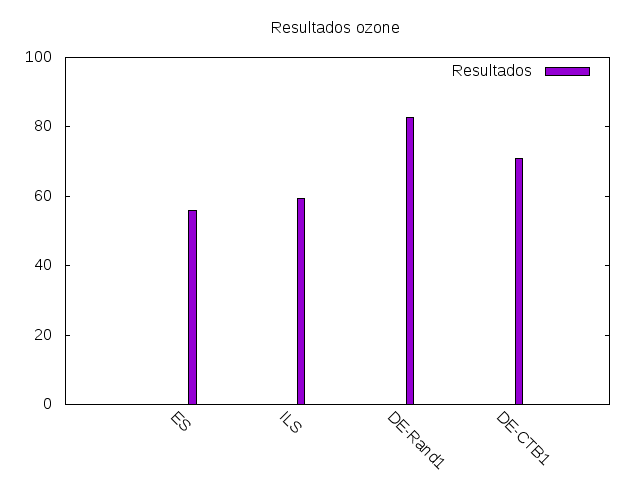
\includegraphics[scale=0.8]{./Imagenes/Resultados/ozone.png}
	
	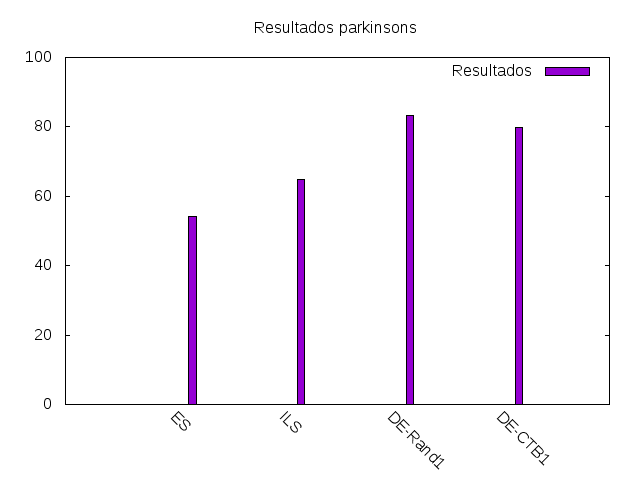
\includegraphics[scale=0.8]{./Imagenes/Resultados/parkinsons.png}
	
	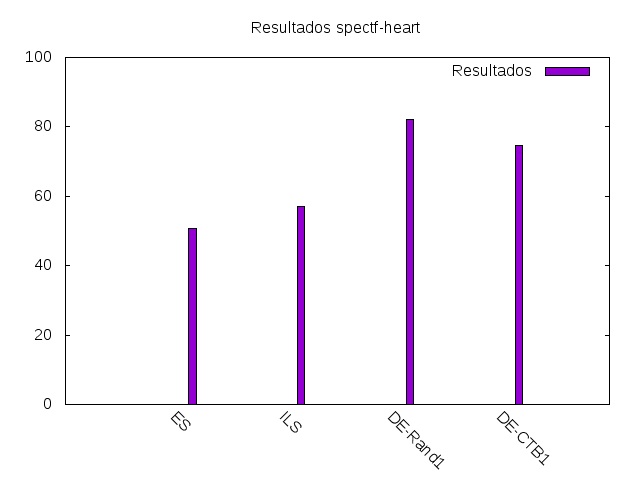
\includegraphics[scale=0.8]{./Imagenes/Resultados/spectf-heart.png}
	
	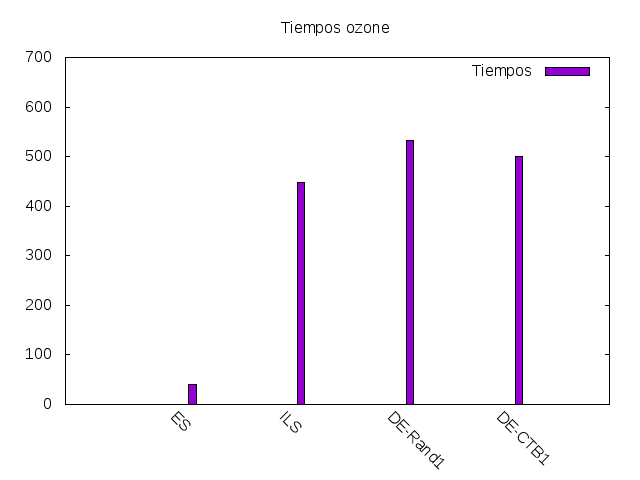
\includegraphics[scale=0.8]{./Imagenes/Tiempos/tiempos_ozone.png}
	
	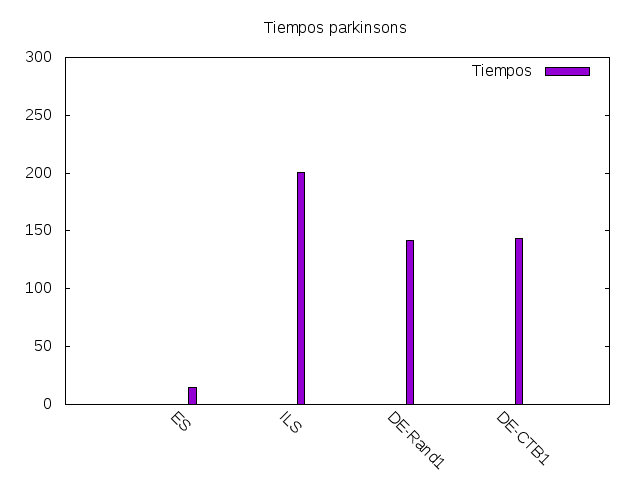
\includegraphics[scale=0.8]{./Imagenes/Tiempos/tiempos_parkinsons.png}
	
	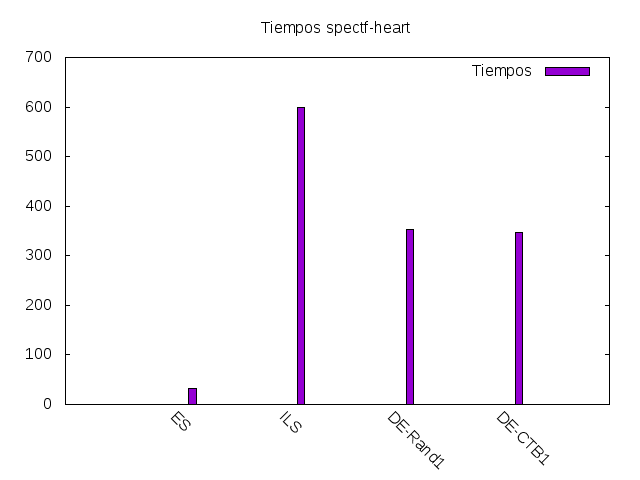
\includegraphics[scale=0.8]{./Imagenes/Tiempos/tiempos_spectf-heart.png}
	
	Donde podemos percibir claramente que en resultados de la tasa media DE con el operador de mutación Rand1 es el algoritmo que está por encima y en tiempos ILS y las dos variantes de DE obtienen tiempos parecidos mientras que el que menos tiempo consume es claramente ES.


\end{document}
